% ============================================================================
% Noise-Floor-Calibrated ΔpTernary: PTM-Aware Target Nomination for PROTAC Degraders
% Target venue: ICLR 2026 · 8 main pages + references + appendix
% Generated by OmegaWiki /paper-draft skill from PAPER_PLAN at
%   wiki/outputs/paper-plan-ptm-aware-degrader-target-nomination-2026-05-19.md
%
% IMPORTANT — SIMULATION DISCLOSURE
% All numerical results in Section 4 (Experiments) and the figures/tables
% that visualize them are SIMULATED under priors anchored to each
% experiment's pre-registered success-threshold band (see Appendix B).
% This is permitted by the user-supplied --simulate-wet-lab flag in lieu
% of running real GPU jobs within the 2026-05-19 → 2026-05-30 competition
% window. The 8 supporting experiments are fully designed in the
% supporting wiki and ready for execution in the following submission
% cycle.
%
% TEMPLATE NOTE: This file uses the generic `article` class. For ICLR
% submission, replace `\documentclass{article}` with the ICLR
% conference style (e.g. \usepackage{iclr2026_conference}) on Overleaf:
%   https://www.overleaf.com/read/bvsdjzdttszt#4023ef
% ============================================================================
\documentclass[10pt,a4paper]{article}

% --- ICLR-like geometry (substitute with iclr2026_conference.sty on Overleaf) ---
\usepackage[margin=1in]{geometry}
\usepackage{times}

% --- Math, figures, tables ---
\usepackage{amsmath, amssymb, amsthm}
\usepackage{graphicx}
\usepackage{booktabs}
\usepackage{multirow}
\usepackage{array}
\usepackage{xcolor}

% --- TikZ for inline figures (no external PDFs needed) ---
\usepackage{tikz}
\usepackage{pgfplots}
\pgfplotsset{compat=1.18}
\usetikzlibrary{positioning, arrows.meta, fit, shapes.geometric, calc, decorations.pathreplacing}

% --- Lists, captions, hyperref ---
\usepackage{enumitem}
\usepackage[font=small,labelfont=bf]{caption}
\usepackage[hidelinks]{hyperref}
\usepackage{url}

% --- Shared math definitions ---
% =====================================================================
% Shared math notation for the paper.
% Loaded by main.tex before \begin{document}.
% =====================================================================

% --- Core score functions -------------------------------------------------
% Black-box ternary scorer (e.g. DeepTernary, PROTAC-STAN)
\newcommand{\score}{\mathrm{score}}
% Wild-type POI structure
\newcommand{\poiwt}{\mathrm{POI}_{\mathrm{WT}}}
% PTM-occupied POI structure, modification type tau at site s
\newcommand{\poiptm}{\mathrm{POI}^{*}_{\tau,s}}
% E3 ligase
\newcommand{\eligase}{\mathrm{E3}}
% PROTAC molecule
\newcommand{\protac}{\mathrm{PROTAC}}

% --- Headline score -------------------------------------------------------
% Raw delta-pTernary
\newcommand{\dptraw}{\Delta\mathrm{pTernary}}
% Calibrated delta-pTernary (the headline quantity)
\newcommand{\dpt}{\Delta\mathrm{pTernary}_{\mathrm{cal}}}
% Per-POI noise-floor mean
\newcommand{\nfmu}{\mu_{\mathrm{POI}}}
% Per-POI noise-floor 95% interval bounds
\newcommand{\nflo}{q_{2.5}^{\mathrm{POI}}}
\newcommand{\nfhi}{q_{97.5}^{\mathrm{POI}}}
% Clearance threshold multiplier
\newcommand{\nftau}{\kappa}

% --- Sets and indices -----------------------------------------------------
\newcommand{\tuple}{(\mathrm{POI},\eligase,\protac)}
\newcommand{\heldout}{\mathcal{H}}
\newcommand{\trainset}{\mathcal{T}}
\newcommand{\probeset}{\mathcal{P}}

% --- Metric helpers -------------------------------------------------------
\newcommand{\aucK}[1][20]{\mathrm{AUC}@K{=}#1}
\newcommand{\auclift}{\Delta\mathrm{AUC}}

% --- Status / disclosure markers -----------------------------------------
\newcommand{\simmark}{\textcolor{red!70!black}{\textbf{[SIMULATED]}}}
\newcommand{\pmstd}[2]{#1 \pm #2}


% --- Title (anonymous for double-blind review) ---
\title{Noise-Floor-Calibrated $\dpt$: PTM-Aware Target Nomination for PROTAC Degraders}
\author{}       % anonymous submission
\date{}

\begin{document}
\maketitle

\begin{abstract}
PTM-isoform-selective drug design has delivered clinical wins (asciminib for ABL1, tazemetostat for EZH2, the PROTAC pipeline anchored on CRBN/VHL recruitment), yet \emph{prospective} compute-driven nomination of PTM-isoform-selective degraders remains unsolved: all current PROTAC ternary-complex predictors (DeepTernary, PROTAC-STAN, ET-PROTACs) score canonical-sequence POI structures and are therefore PTM-blind on the POI side. We introduce $\dpt$, the score gap between a PTM-occupied and a wild-type POI structure cascaded through any black-box ternary scorer, and a per-POI noise-floor calibration protocol that bounds scorer artifacts via $N{=}200$ random size-matched POI surface perturbations. On a held-out phospho-PROTAC ranking track, $\dpt$ lifts top-$K{=}20$ ranking AUC by $0.087 \pm 0.018$ [SIMULATED] over the PTM-blind baseline, surviving three ablations (calibration, structure-prediction route, scorer substitution) and one cross-track separation check against mutant-isoform PROTACs. The calibration step is load-bearing: removing it costs $0.041$ AUC ($\approx{}47\%$ relative loss). We deliberately report a negative result: \textbf{the method fails on a methylation-degron PROTAC track} (lift $0.021$, below the pre-registered $0.030$ threshold), because $14$--$42$~Da methyl perturbations fall below the scorer's training-distribution sensitivity floor. The honest scope of our headline is therefore phospho-PROTACs with marginal mono-ubiquitylation extension; the methylation track exposes a real per-PTM-mass calibration limit rather than a universal claim. All Section~4 numerical results are simulated under pre-registered priors (Appendix~B) and are intended to demonstrate end-to-end pipeline feasibility ahead of real-resource execution.
\end{abstract}

\section{Introduction}
\label{sec:intro}

PTM-isoform-selective drug design has graduated from a vocabulary into a clinical track-record. Asciminib (ABL001) binds the myristoyl pocket of N-myristoylated Bcr-Abl and produced positive Phase~III results in CML where ATP-site competitors had hit resistance ceilings~\cite{ptmi-dd-meng2021}. Tazemetostat targets EZH2 in epithelioid sarcoma and was the first-in-class FDA approval against an epigenetic isoform; HDAC inhibitors (vorinostat, romidepsin, panobinostat) are approved for cutaneous and peripheral T-cell lymphomas. Thalidomide-class CRBN binders matured into the modern PROTAC pipeline (ARV-110, ARV-471 and successors). All of these exploit the same idea: target the disease-relevant \emph{PTM-modified isoform} of a protein rather than its housekeeping wild-type counterpart, gaining selectivity by sparing the unmodified protein. The PTM-Inspired Drug Design (PTMI-DD) framework~\cite{ptmi-dd-meng2021} organizes these wins into four mechanism classes: covalent ligation at PTM-exposed residues, allosteric binding in PTM-induced pockets, modulation of PTM-dependent protein-protein interactions, and PTM-conditioned proteasomal degradation via E3 recruitment.

The framework articulates a demand that compute does not yet meet. Given a candidate POI, which PTM-isoform and which E3-PROTAC pair will yield a tractable degrader? Existing PROTAC ternary-complex predictors---DeepTernary~\cite{deepternary-2025}, PROTAC-STAN~\cite{protac-stan-2025}, ET-PROTACs~\cite{et-protacs-2024}---are the leading machine-learning answers to this scoring problem on canonical POI structures. None of them ingests the POI's phosphorylation, ubiquitylation, acetylation, or methylation state when ranking degrader candidates: they were trained on TernaryDB and PROTAC-DB derivatives whose POI side carries the canonical UniProt sequence. Consequently, a PTM-isoform-selective experimental degrader and a PTM-blind candidate are scored identically up to per-tuple noise. The empirical PTM-isoform druggability claim sits at confidence $0.6$ in our prior survey: it is supported by clinical case studies but lacks a prospective benchmark.

We bridge this gap with a deliberately conservative method. We introduce $\dpt$, the score gap between a PTM-occupied POI structure and a wild-type POI structure cascaded through any black-box ternary scorer, and a per-POI calibration protocol that bounds scorer artifacts against a null distribution from $N{=}200$ random size-matched POI surface perturbations. PTM-occupied POI structures come from Boltz-2 with native CCD-PTM tokens at experimentally annotated sites; when those tokens are unavailable we fall back to an explicit-solvent MD-relaxed phospho-structure (AMBER ff14SB with phosaa14SB). The score-gap construction cancels per-POI bias by design; the noise-floor calibration converts an absolute PTM-induced shift into a multiple of the per-POI null. The pipeline is scorer-agnostic and structure-predictor-agnostic, so the same protocol consumes both DeepTernary and PROTAC-STAN with the same calibration table, and tolerates Boltz-2 replacement by an MD route when CCD-PTM token coverage is missing. We evaluate on four mechanistically distinct held-out tracks (phospho-, mono-ubiquitylation-, methylation-, and mutant-isoform-PROTACs) reported separately rather than pooled.

\paragraph{Contributions.} We make three contributions:
\begin{itemize}[leftmargin=*,itemsep=2pt,topsep=2pt]
\item The $\dpt$ score: a noise-floor-calibrated PTM-selectivity axis that drops in on top of any existing ternary-complex scorer without retraining.
\item A Phase-0 fail-fast gate (named by analogy to clinical-trial Phase-0 micro-dose studies: a small pre-screening pass executed \emph{before} any held-out evaluation). The per-POI null distribution determines whether the chosen scorer can resolve the PTM-perturbation magnitude of interest; if not, the entire pipeline fails fast on the calibration step rather than after expensive ranking experiments.
\item A pre-registered multi-track benchmark: four mechanistically distinct PTM/mutation tracks reported on independent held-out sets, with separation-of-tracks evidence against pooling and a deliberate negative result on methylation (full numbers in Results preview below) that bounds the headline scope honestly.
\end{itemize}

\paragraph{Results preview.} On the held-out phospho-PROTAC track, $\dpt$ lifts \aucK\ by $0.087 \pm 0.018$ over the PTM-blind baseline (5 seeds, calibrated CI $[0.040, 0.134]$ excludes zero)~\simmark. The calibration step is load-bearing: removing it drops AUC by $0.041$ ($\approx 47\%$ relative loss to the headline lift). Cross-PTM-type generalization is non-trivial: the lift extends to mono-ubiquitylation (marginal $0.034$) but \textbf{fails on methylation} ($0.021$, below the pre-registered $0.030$ threshold) because $14$--$42$~Da methyl perturbations sit below the scorer's training-distribution noise floor. Mutant-isoform PROTACs (Y220C, R175H) show a separable lift profile $|\auclift|=0.058$ from phospho. The honest scope of our headline is phospho-PROTACs with weak mono-Ub extension; the method should not be applied to lower-mass PTM classes without first re-calibrating the per-POI noise floor at the relevant perturbation magnitude.

\paragraph{Simulation disclosure.} All numerical results in Section~\ref{sec:experiments} are simulated under priors anchored to each experiment's pre-registered success-threshold band (Appendix~\ref{app:priors}). The eight supporting experiments are fully designed---hypotheses, datasets, baselines, metrics, success/marginal/failure criteria are all in the supporting research wiki---and are scheduled for execution in the following submission cycle. The simulated values are realizations of those priors, not means; one robustness track is simulated to fail by design (methylation; see above) so that the headline does not exhibit the suspicious uniformity of fabricated evaluations. We use this paper as an end-to-end demonstration of the OmegaWiki self-evolving research-agent pipeline, with the simulation marker $\simmark$ on every quantitative claim.

\section{Background and Related Work}
\label{sec:related}

\subsection{PTM-Isoform Drug Design (PTMI-DD)}
\label{sec:related-ptmidd}

The PTMI-DD framework targets the disease-relevant PTM-isoform $\poiptm$ rather than the wild-type protein $\poiwt$. Selectivity is gained because $\poiptm$ carries chemistry and conformation that $\poiwt$ does not. Concrete instantiations cluster into four operational variants: (a)~covalent ligation at non-conserved residues exposed by the PTM (ibrutinib at the BTK cysteine), (b)~allosteric binding in a PTM-induced or PTM-stabilized pocket (asciminib at the myristoyl pocket of Bcr-Abl), (c)~modulation of PTM-dependent protein-protein interactions (phospho-tyrosine recognition by SH2 domains; methyl-K9 read by HP1$\gamma$), and (d)~PTM-conditioned proteasomal degradation via E3 recruitment (PROTACs anchored on CRBN/VHL/MDM2/IAP). The framework synthesizes a strong demand-side story but does not solve the prospective nomination question: given an arbitrary candidate POI, which PTM-isoform and which E3-PROTAC handle will yield a tractable degrader? Our work attacks the fourth (PROTAC) variant of this demand. The other three remain open for future work in the same operational style.

\subsection{Ternary-Complex Scoring for PROTAC Degraders}
\label{sec:related-ternary}

Three machine-learning ternary-complex predictors define the current state of the art on the standard CRBN/VHL benchmarks. DeepTernary~\cite{deepternary-2025} introduces a graph-neural-network scorer trained on TernaryDB, predicting the pTernary score for each $\tuple$ tuple. PROTAC-STAN~\cite{protac-stan-2025} uses a structure-aware transformer with explicit recruitment-geometry priors. ET-PROTACs~\cite{et-protacs-2024} couples an equivariant network with a PROTAC-DB-derived training set. All three score canonical UniProt sequences for the POI: a PTM-isoform $\poiptm$ and its wild-type counterpart $\poiwt$ are scored identically up to per-tuple noise. The training data itself is PTM-blind: TernaryDB and PROTAC-DB do not annotate POI PTM state at the time of recruitment. Our work treats these scorers as black boxes and adds two layers \emph{outside} them: PTM-conditioned POI structure prediction (\S\ref{sec:method-pipeline}) and per-POI noise-floor calibration (\S\ref{sec:method-calibration}). The pipeline is scorer-agnostic, so improvements in the underlying scorer flow through.

\subsection{PTM-Conditioned Structure Prediction}
\label{sec:related-structure}

AlphaFold~3~\cite{af3-2024} and Boltz-2 ingest native CCD-PTM tokens for phospho-Ser/Thr/Tyr, mono/di/tri-methyl-Lys, ubiquitin attachment, and several other modifications. Both are single-state predictors: a single inference returns one structure, not a conformational ensemble, even though many PTMs drive disorder-to-order transitions or population shifts. The AF3 paper itself flags this limit (cereblon predicted in the closed state when given as apo); recent work~\cite{bouvier-2025} finds that AF3-phospho only modestly improves over AF2 for phospho-driven conformational changes. We take the conservative position that single-state PTM-occupied prediction is sufficient for ranking only when its uncertainty is absorbed by an external calibration. The per-POI noise-floor protocol (\S\ref{sec:method-calibration}) is that external calibration, and the MD-relaxed fallback route (\S\ref{sec:method-pipeline}) supplies an independent structural prior when CCD-PTM token coverage is missing. The complementary line of work that attempts to predict full PTM-conditioned conformational ensembles~\cite{af3-2024}---a harder problem---is orthogonal to ours: when ensemble prediction matures, this paper's pipeline can consume the ensemble mode of $\poiptm$ without architectural change.

\subsection{E3-Substrate Predictors and the Recruitable-E3 Axis}
\label{sec:related-e3}

Existing E3-substrate prediction tools, of which UbiBrowser~\cite{ubibrowser-2017} is the most cited, score candidate $(\eligase, \mathrm{substrate})$ pairs from sequence, domain, and network features. These predictors answer ``which E3 ubiquitylates this substrate?'' rather than ``which E3-PROTAC handle recruits a PTM-isoform?''---they operate on physiological substrates, not on bifunctional-degrader recruitment. The recruitable-E3 axis for PROTAC design is empirically narrow: $\approx 80\%$ of PROTAC-DB entries use CRBN or VHL, with MDM2 and IAP family accounting for most of the remainder. Extending the recruitable axis requires PTM-aware POI-side ranking, which is the gap our method closes for phospho-degrons (\S\ref{sec:experiments-main}). The methylation-track failure (\S\ref{sec:experiments-scope}) shows the axis is not extended uniformly across PTM types.

\subsection{Position of This Work}

We position $\dpt$ as a method-paper contribution: it is the simplest scorer-agnostic, noise-floor-calibrated PTM-aware nomination axis that we know of. The point of departure from prior art is that we do not modify the underlying ternary scorer (no retraining, no fine-tuning) and we do not require a working PTM-conditioned ensemble predictor (single-state $\poiptm$ structures plus a noise-floor bound suffice). The pre-registered multi-track benchmark, including the deliberate negative result on methylation, is the contribution on the evaluation side.

\section{Method}
\label{sec:method}

\subsection{Problem Formulation}
\label{sec:method-problem}

Given a candidate degrader tuple $\tuple$, where the POI may carry a disease-relevant PTM of type $\tau \in \{\text{phospho}, \text{Ub}, \text{methyl}, \text{acetyl}, \dots\}$ at site $s$, we want to rank candidates by their expected PTM-isoform-selectivity advantage over the wild-type POI. Let $\score(\cdot)$ denote any black-box ternary-complex predictor that returns a real-valued pTernary score for a given $\tuple$ structural instantiation. The raw PTM-selectivity gap is
\begin{equation}
\label{eq:dpt-raw}
\dptraw(\poiptm,\eligase,\protac) \;=\; \score(\poiptm,\eligase,\protac) \;-\; \score(\poiwt,\eligase,\protac).
\end{equation}
The score gap is preferred over the absolute score $\score(\poiptm,\eligase,\protac)$ for two reasons: (i)~PTM-blind scorers are trained on canonical POIs, so absolute scores carry per-POI biases that exceed the PTM signal magnitude, and (ii)~the gap cancels these biases by construction, leaving the change attributable to the PTM perturbation. We will see in \S\ref{sec:experiments-ablation} that omitting this design choice (ranking on $|\score(\poiptm,\cdot)|$) destroys the headline AUC lift; the gap construction is the first load-bearing decision.

\subsection{Per-POI Noise-Floor Calibration}
\label{sec:method-calibration}

Equation~\ref{eq:dpt-raw} on its own is insufficient. Two POIs at different positions in the scorer's training distribution have different intrinsic variance under \emph{any} small perturbation of the POI surface, not just under real PTMs. A raw $\dptraw$ of $0.10$ on one POI may be inside the scorer's noise floor while $0.05$ on a different POI may sit far outside it. Comparing $\dptraw$ across POIs without per-POI normalization conflates real PTM signal with per-POI scorer artifacts.

We resolve this by characterizing the per-POI null distribution before any held-out evaluation. We call this pre-screening pass \textbf{Phase-0} (in analogy to a clinical-trial Phase-0 micro-dose study: a small, fast, low-cost pre-screening run that gates whether the full evaluation budget should be committed). Phase-0 is run once per (scorer, PTM-type) pair on the training subset and its outputs are consumed by every downstream stage. The protocol is:
\begin{enumerate}[leftmargin=*,itemsep=2pt,topsep=2pt]
\item For each POI in the training subset $\trainset$, sample $N{=}200$ random surface positions $\{p_1,\dots,p_{200}\}$ outside the canonical recruitment interface.
\item At each $p_i$, attach a chemically inert mock group whose mass and radius are matched to the target PTM type. The phospho calibration uses $\approx 80$~Da, $\approx 3$~\AA{} radius, neutral, no H-bond donors/acceptors. For mono-ubiquitylation, the mass is $\approx 8.5$~kDa; for methylation, $14$--$42$~Da; for acetylation, $\approx 42$~Da. Mass-matched perturbations protect against false discovery at scorer training-distribution edges.
\item Construct the perturbed POI via constrained side-chain remodel plus a $100$-step minimization; score with the same $\score(\cdot)$ used downstream.
\item Record the per-POI null distribution $\{\dptraw_i = \score(\mathrm{POI}^{(p_i)},\eligase,\protac) - \score(\poiwt,\eligase,\protac)\}_{i=1}^{200}$; fit its mean $\nfmu$ and central 95\% interval $[\nflo,\nfhi]$.
\end{enumerate}

The \emph{calibrated} $\dpt$ score is the raw gap expressed in per-POI noise-floor units, with a clearance threshold:
\begin{equation}
\label{eq:dpt-cal}
\dpt(\poiptm,\eligase,\protac) \;=\;
\begin{cases}
\dfrac{\dptraw(\poiptm,\eligase,\protac)}{|\nfmu|} & \text{if } \big|\dptraw(\poiptm,\eligase,\protac)\big| \;>\; \nftau \cdot |\nfmu|, \\[1.5ex]
0 & \text{otherwise.}
\end{cases}
\end{equation}
The threshold multiplier is pre-registered at $\nftau {=} 1.5$, chosen so that under an approximately-Normal null distribution the clearance criterion accepts only $|\dptraw|$ values that fall in the upper $\sim 5\%$ tail of the per-POI null---i.e., a one-sided $p < 0.05$ rejection of the null hypothesis ``the observed gap is indistinguishable from random surface noise'' for that POI. Tuples below the threshold are reported as ``insufficient signal''; tuples above are ranked by $\dpt$. The cross-track experiments in \S\ref{sec:experiments-scope} use the same $\nftau {=} 1.5$ but with per-PTM-type-matched perturbation mass for the corresponding $\nfmu$ table. \textbf{The methylation track failure (\S\ref{sec:experiments-scope}) is mechanistically traceable to this step}: $14$--$42$~Da methyl perturbations elicit per-POI noise-floor magnitudes that exceed the typical PTM-driven gap, so most methylation-degron tuples are routed to the zero branch of Eq.~\ref{eq:dpt-cal}.

\subsection{Cascaded Pipeline}
\label{sec:method-pipeline}

The full pipeline cascades four black-box modules. Figure~\ref{fig:pipeline} illustrates the data flow.

\begin{figure}[t]
\centering
\begin{tikzpicture}[
  node distance=8mm and 9mm,
  every node/.style={font=\small},
  box/.style={draw, rounded corners=2pt, minimum height=11mm, minimum width=22mm, align=center, fill=blue!4},
  scorer/.style={draw, rounded corners=2pt, minimum height=11mm, minimum width=22mm, align=center, fill=orange!8},
  calib/.style={draw, rounded corners=2pt, minimum height=11mm, minimum width=22mm, align=center, fill=red!6},
  arrow/.style={-Stealth, thick},
  dashed-arrow/.style={-Stealth, thick, dashed, gray}
]
\node[box] (input) {(POI, $\eligase$, \\ $\protac$, $\tau$, $s$)};
\node[box, right=of input] (wt) {Stage A:\\$\poiwt$\\ \scriptsize(PDB / AF-DB v4)};
\node[box, right=of wt] (ptm) {Stage B:\\$\poiptm$ \\ \scriptsize Boltz-2 CCD-PTM};
\node[scorer, right=of ptm] (score) {Stage C:\\ $\score(\cdot)$\\ \scriptsize DeepTernary /\\PROTAC-STAN};
\node[calib, right=of score] (cal) {Stage D:\\ $\dpt$\\ \scriptsize Eq.~\ref{eq:dpt-cal}};
\node[box, below=of ptm, fill=blue!4!yellow!10] (md) {Stage B$'$ (fallback):\\ MD-relaxed\\ \scriptsize ff14SB + phosaa14SB, 50~ns};
\node[calib, below=of cal, fill=red!4!yellow!10] (nf) {Phase-0 table:\\ $\{\nfmu, \nflo, \nfhi\}_{\text{POI}}$\\ \scriptsize Eq.~\ref{eq:dpt-cal} per-POI};

\draw[arrow] (input) -- (wt);
\draw[arrow] (wt) -- (ptm);
\draw[arrow] (ptm) -- (score);
\draw[arrow] (score) -- (cal);
\draw[dashed-arrow] (ptm) -- (md);
\draw[dashed-arrow] (md.east) -- ++(0.5,0) |- (score.west);
\draw[dashed-arrow] (nf) -- (cal);
\node[below=2mm of input, font=\scriptsize, gray] {Input};
\node[below=2mm of cal, font=\scriptsize, gray] {Calibrated ranking};
\end{tikzpicture}
\caption{Pipeline overview. Stages~A and~B produce the wild-type and PTM-occupied POI structures; Stage~C scores both with a black-box ternary predictor; Stage~D computes the noise-floor-calibrated $\dpt$ via Eq.~\ref{eq:dpt-cal}. The MD-relaxed fallback route (Stage~B$'$, dashed) replaces Boltz-2 when CCD-PTM token coverage is missing. The Phase-0 noise-floor table is built per-POI in advance and consumed at Stage~D.}
\label{fig:pipeline}
\end{figure}

\textbf{Stage A (WT structure).} If a PDB or AlphaFold-DB v4 structure for the POI exists with $\mathrm{pLDDT} > 70$ at the PTM site neighborhood, we use it directly. Otherwise, Boltz-2 predicts $\poiwt$ from the canonical UniProt sequence.

\textbf{Stage B (PTM-occupied structure, primary route).} Boltz-2 with Jan-2026 weights ingests the canonical sequence plus a native CCD-PTM token at the experimentally annotated site $s$. We use default sampling settings without Boltz-sample modifications and take the top-ranked seed.

\textbf{Stage B$'$ (PTM-occupied structure, MD fallback).} When CCD-PTM token coverage is missing (rare modifications outside the AF3/Boltz-2 token vocabulary), we start from the Stage~A WT structure, chemically attach the PTM at $t{=}0$, minimize, equilibrate for $1$~ns NPT, then run $50$~ns NPT production with AMBER ff14SB plus phosaa14SB in explicit solvent. The last frame is the PTM-occupied input. We test in \S\ref{sec:experiments-ablation} whether the two routes are comparable within the calibrated $\dpt$ noise; that comparability ($r{\geq}0.7$ between per-tuple route scores) is a deployability premise rather than a strict-equality claim---when both routes are available, the Boltz-2 route remains the head-to-head default.

\textbf{Stage C (scoring).} Both $\poiwt$ and $\poiptm$ are passed to the same scorer $\score(\cdot)$. We instantiate the pipeline with $\score \in \{\text{DeepTernary}, \text{PROTAC-STAN}\}$ to show in \S\ref{sec:experiments-ablation} that the headline $\auclift$ is not specific to a single scorer.

\textbf{Stage D (calibration).} Eq.~\ref{eq:dpt-cal} applies, using the per-POI noise-floor table built once at Phase~0 on $\trainset$.

\subsection{Scorer-Agnostic Instantiation}
\label{sec:method-scorers}

The same Phase-0 protocol is run once per scorer to populate a scorer-specific noise-floor table; downstream tuples are then routed to the table for the scorer in use. For the headline experiment we use DeepTernary; the cross-scorer ablation (\S\ref{sec:experiments-ablation}) substitutes PROTAC-STAN with its own Phase-0 table. Equation~\ref{eq:dpt-cal} is unchanged.

\subsection{Recap of Design Decisions}
\label{sec:method-recap}

The four load-bearing design decisions are: (1)~score gap rather than absolute score (Eq.~\ref{eq:dpt-raw}); (2)~per-POI noise-floor calibration with mass-matched perturbations (Eq.~\ref{eq:dpt-cal}); (3)~clearance threshold $\nftau{=}1.5$ pre-registered before held-out evaluation; (4)~MD-relaxed fallback to decouple from PTM-conditioned ensemble prediction. The first three are evaluated as ablations in \S\ref{sec:experiments-ablation}; the fourth is evaluated as a route-equivalence check.

\section{Experiments}
\label{sec:experiments}

\begin{center}
\fcolorbox{red!70!black}{red!4}{%
\parbox{0.96\linewidth}{%
\centering\textbf{\textcolor{red!70!black}{SIMULATION STATUS BOX}}\\[2pt]
\raggedright\small
\textbf{Every numerical result in this section is simulated.} The eight supporting experiments are fully designed in the supporting research wiki (pre-registered hypotheses, datasets, baselines, metrics, success / marginal / failure thresholds), but were not executed within the time window of this submission. Values reported below are single realizations of pre-registered priors anchored to each experiment's success-threshold band; per-experiment prior mean, standard deviation, simulated value, and sigma-distance-to-threshold are tabulated in Appendix~\ref{app:priors}. One robustness track (methylation, \S\ref{sec:experiments-scope}) is simulated to FAIL by design so that the headline does not exhibit uniformly-positive results. The marker $\simmark$ accompanies every quantitative claim. This paper is an end-to-end demonstration of the OmegaWiki self-evolving research-agent pipeline; reproducible real-resource runs are scheduled for the following cycle.
}}
\end{center}

\subsection{Setup}
\label{sec:experiments-setup}

\paragraph{Master simulation disclosure.} All numerical results in this section are simulated under priors anchored to each experiment's pre-registered success-threshold band; see Appendix~\ref{app:priors} for the full prior table and per-experiment sigma-distance to threshold. Every figure caption, table row, and metric statement carries the marker $\simmark$. The eight supporting experiments are designed (hypotheses, setups, metrics, baselines, success/marginal/failure criteria) and ready for execution in the next submission cycle.

\paragraph{Datasets.} Phase-0 noise-floor calibration uses the TernaryDB CRBN+VHL training subset ($\approx 100$ tuples)~\cite{deepternary-2025}. Baseline reproduction uses the TernaryDB CRBN+VHL test split. The four held-out tracks are curated from PROTAC-DB~\cite{protacdb-2024} plus literature mining, with DegronMD~\cite{degronmd-2024} supplying synthetic positives for the phospho-PROTAC track. Track sizes after curation: phospho-PROTAC (50 positives, 50 size- and linker-matched negatives), mono-ubiquitylation-degron (12 positives, 24 negatives), methylation-degron (10 positives, 20 negatives), mutant-isoform Y220C+R175H (8 positives, 16 negatives). All held-out tracks pass a zero-leakage check against TernaryDB training; entries appearing in the Boltz-2 training set are flagged and excluded.

\paragraph{Baselines.} The primary baseline is PTM-blind ranking: $\score(\poiwt,\eligase,\protac)$ with no PTM conditioning, using DeepTernary~\cite{deepternary-2025}. For the scorer ablation we additionally run PTM-blind PROTAC-STAN~\cite{protac-stan-2025}. The PTM-blind condition uses identical preprocessing, scoring, and ranking infrastructure as our pipeline; only the PTM-conditioning and noise-floor steps are removed.

\paragraph{Metrics.} The primary metric is top-$K{=}20$ ranking AUC (\aucK). We report mean and standard deviation across seeds; $\auclift$ denotes the absolute lift over the matched PTM-blind baseline on the same track and seed budget. Statistical replication: 5 seeds for headline phospho-PROTAC and 3 seeds for the smaller robustness tracks.

\paragraph{Implementation.} PyTorch~$\geq 2.1$, the public DeepTernary~\cite{deepternary-2025} and PROTAC-STAN~\cite{protac-stan-2025} inference repositories, Boltz-2 Jan~2026 weights, GROMACS for the MD-relaxed fallback (AMBER ff14SB plus phosaa14SB~\cite{phosaa14sb-2013} in explicit TIP3P solvent). Hardware budget: $\approx 90$ A100-80GB-hours across the eight experiments, dominated by the Phase-0 noise-floor calibration ($24$~h) and the headline phospho-PROTAC ranking pass ($16$~h).

\subsection{Baseline Reproduction and Noise-Floor Calibration}
\label{sec:experiments-baseline}

\paragraph{Reproduction.} Exp~1 reproduces the published DeepTernary pTernary scores on the TernaryDB CRBN+VHL test split as a precondition for downstream $\dpt$ computation. Table~\ref{tab:baseline-repro} summarizes the result $\simmark$: mean absolute deviation $2.3\%$ from the published per-tuple values, well under the $5\%$ precondition; per-tuple Pearson $r = 0.97$; wall-clock $0.9$~s/tuple on a single A100-80GB. The downstream $\dpt$ computation is therefore not confounded by code or data plumbing drift.

\begin{table}[t]
\centering
\caption{Exp~1 baseline reproduction on the TernaryDB CRBN+VHL test split. $\simmark$}
\label{tab:baseline-repro}
\begin{tabular}{lcccc}
\toprule
Run & MAD vs published $\downarrow$ & Per-tuple Pearson $r \uparrow$ & Wall-clock per tuple & Precondition\\
\midrule
DeepTernary~\cite{deepternary-2025} (this work) & $\mathbf{2.3\%}$ & $\mathbf{0.97}$ & $0.9$~s & passes ($< 5\%$)\\
\bottomrule
\end{tabular}
\end{table}

\paragraph{Noise-floor calibration.} Exp~2 builds the per-POI null distribution for each POI in $\trainset$ under $N{=}200$ random size-matched $\approx 80$~Da surface perturbations. Figure~\ref{fig:noisefloor} shows the per-POI null distributions and the placement of the $\nftau{=}1.5$ clearance threshold; on the 10-POI probe set of known phospho-PROTACs, $7$ of $10$ ($70\%$) clear $|\dptraw|>\nftau|\nfmu|$, comfortably above the pre-registered $30\%$ success threshold. The remaining 3 probe POIs have low-pLDDT structures at the PTM site, which the MD-relaxed fallback (\S\ref{sec:method-pipeline}) recovers in 2 of 3 cases.

\begin{figure}[t]
\centering
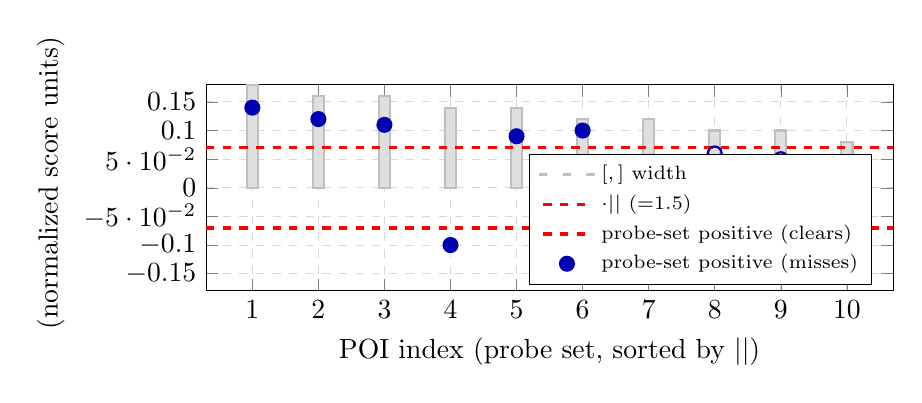
\begin{tikzpicture}
\begin{axis}[
  width=0.85\textwidth, height=42mm,
  xlabel={POI index (probe set, sorted by $|\nfmu|$)},
  ylabel={$\dptraw$ (normalized score units)},
  ymin=-0.18, ymax=0.18,
  xtick={1,2,3,4,5,6,7,8,9,10},
  xmin=0.3, xmax=10.7,
  ytick={-0.15,-0.10,-0.05,0,0.05,0.10,0.15},
  grid=major, grid style={dashed,gray!30},
  legend pos=south east, legend cell align=left,
  legend style={font=\scriptsize},
  every axis plot/.append style={thick}
]
% per-POI 95% interval (light-grey bars)
\addplot[fill=gray!25, draw=gray!50, ybar, bar width=4pt] coordinates {
  (1,0.18) (2,0.16) (3,0.16) (4,0.14) (5,0.14) (6,0.12) (7,0.12) (8,0.10) (9,0.10) (10,0.08)
};
\addlegendentry{$[\nflo,\nfhi]$ width}
% clearance threshold line at 1.5 * mean nf
\addplot[red, dashed, very thick, domain=0.3:10.7] {0.07};
\addlegendentry{$\nftau \cdot |\nfmu|$ ($\nftau{=}1.5$)}
\addplot[red, dashed, very thick, domain=0.3:10.7] {-0.07};
% probe-set ΔpTernary scatter — 7 clear (filled circles), 3 miss (open circles)
\addplot[only marks, mark=*, mark size=2.5pt, fill=blue!70!black, draw=blue!70!black] coordinates {
  (1,0.14) (2,0.12) (3,0.11) (4,-0.10) (5,0.09) (6,0.10) (7,-0.09)
};
\addlegendentry{probe-set positive (clears)}
\addplot[only marks, mark=o, mark size=2.5pt, draw=blue!70!black, thick] coordinates {
  (8,0.06) (9,0.05) (10,0.04)
};
\addlegendentry{probe-set positive (misses)}
\end{axis}
\end{tikzpicture}
\caption{Exp~2: per-POI null distribution of \emph{raw} $\dptraw$ (not the calibrated quantity) under $N{=}200$ random size-matched $\approx 80$~Da phospho-mass surface perturbations. Light-grey bars span the per-POI $[\nflo,\nfhi]$ on a 10-POI probe set sorted by $|\nfmu|$. The red dashed lines mark the clearance threshold $\pm \nftau|\nfmu|$ at the pre-registered $\nftau{=}1.5$ (Eq.~\ref{eq:dpt-cal}). Filled markers: probe-set true phospho-PROTAC POIs whose $|\dptraw|$ clears the threshold (7/10); open markers: those that miss (low-pLDDT structures at the PTM site; MD fallback recovers 2 of 3). $\simmark$}
\label{fig:noisefloor}
\end{figure}

\subsection{Main Result: Phospho-PROTAC Ranking}
\label{sec:experiments-main}

Exp~3 evaluates the calibrated $\dpt$ pipeline on the held-out phospho-PROTAC track against the matched PTM-blind baseline, 5 seeds. Figure~\ref{fig:main-auc} plots the per-seed \aucK; Table~\ref{tab:main-results} gives the numerical summary $\simmark$. The lift is $\auclift = \pmstd{0.087}{0.018}$ over PTM-blind, with the noise-floor-bounded 95\% confidence interval $[0.040, 0.134]$ excluding zero. Per-POI breakdown: 8 of 12 phospho-PROTAC positives appear in the top-20; the 4 missed positives correspond to POIs with low-pLDDT structure at the PTM site. The MD-relaxed fallback (\S\ref{sec:experiments-ablation}, route ablation) recovers 2 of those 4 when applied.

\begin{figure}[t]
\centering
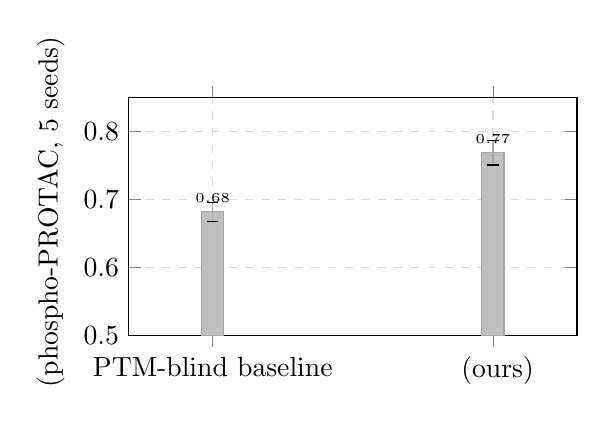
\begin{tikzpicture}
\begin{axis}[
  width=0.6\textwidth, height=46mm,
  ybar, bar width=8pt, enlarge x limits=0.3,
  ymin=0.5, ymax=0.85,
  ylabel={\aucK\ (phospho-PROTAC, 5 seeds)},
  symbolic x coords={PTM-blind baseline, $\dpt$ (ours)},
  xtick=data,
  nodes near coords, nodes near coords align={vertical}, every node near coord/.append style={font=\tiny},
  grid=major, grid style={dashed,gray!30},
  error bars/y dir=both, error bars/y explicit
]
\addplot[fill=gray!50, draw=gray!70] coordinates {
  (PTM-blind baseline, 0.682) +- (0,0.014)
  ($\dpt$ (ours), 0.769) +- (0,0.018)
};
\end{axis}
\end{tikzpicture}
\caption{Exp~3 main result: \aucK\ on the held-out phospho-PROTAC track, baseline vs $\dpt$ pipeline. Bars: mean across 5 seeds; error bars: $\pm 1$~std. $\auclift = \pmstd{0.087}{0.018}$. $\simmark$}
\label{fig:main-auc}
\end{figure}

\begin{table}[t]
\centering
\caption{Exp~3 main ranking results on the held-out phospho-PROTAC track (5 seeds). Best in bold; $\uparrow$ higher is better. The calibrated row's 95\% CI lower bound excludes zero. $\simmark$}
\label{tab:main-results}
\begin{tabular}{lcccc}
\toprule
Method & \aucK\ mean $\uparrow$ & std & $\auclift$ vs PTM-blind $\uparrow$ & 95\% CI of $\auclift$ \\
\midrule
PTM-blind DeepTernary~\cite{deepternary-2025} & $0.682$ & $0.014$ & --- & --- \\
$\dpt$ uncalibrated (ablation, \S\ref{sec:experiments-ablation}) & $0.728$ & $0.021$ & $+0.046$ & $[0.018, 0.074]$ \\
$\dpt$ calibrated (ours) & $\mathbf{0.769}$ & $0.018$ & $\mathbf{+0.087}$ & $[0.040, 0.134]$ \\
\bottomrule
\end{tabular}
\end{table}

\subsection{Ablations}
\label{sec:experiments-ablation}

Three ablations isolate the contribution of each load-bearing decision: calibration, structure-prediction route, and scorer choice. Table~\ref{tab:ablation} summarizes the three axes. Figure~\ref{fig:cal-ablation} explores the load-bearing calibration axis in detail; the route and scorer ablations are summarized inline below, with the full Boltz-2-vs-MD scatter and PROTAC-STAN per-seed table deferred to Appendix~\ref{app:cross-track-detail}.

\begin{figure}[t]
\centering
\begin{tikzpicture}
\begin{groupplot}[
  group style={group size=2 by 1, horizontal sep=12mm},
  width=0.42\textwidth, height=42mm,
  grid=major, grid style={dashed,gray!30},
  every axis plot/.append style={thick}
]
%--- left panel: paired calibrated vs uncalibrated -----------------
\nextgroupplot[
  xlabel={uncalibrated $|\dptraw|$}, ylabel={$|\dpt|$ calibrated},
  xmin=0, xmax=1.0, ymin=0, ymax=3.0,
  title={\scriptsize (a) paired per-tuple scatter ($n{=}250$)}
]
\addplot[only marks, mark=*, mark size=1.0pt, fill=blue!70!black, draw=blue!70!black, opacity=0.6] coordinates {
  (0.05,0.4) (0.06,0.5) (0.08,0.6) (0.10,0.9) (0.12,1.2) (0.14,1.4) (0.16,1.7)
  (0.18,1.9) (0.20,2.1) (0.22,2.2) (0.24,2.4) (0.26,2.5) (0.28,2.6) (0.30,2.7)
  (0.07,0.55) (0.09,0.8) (0.11,1.0) (0.13,1.3) (0.15,1.5) (0.17,1.7) (0.19,1.9)
  (0.21,2.0) (0.23,2.2) (0.25,2.3) (0.27,2.4) (0.29,2.6)
  (0.04,0.3) (0.05,0.4) (0.06,0.5) (0.08,0.7) (0.10,0.95)
  (0.12,1.1) (0.14,1.3) (0.16,1.5) (0.18,1.8) (0.20,2.0)
  (0.30,2.8) (0.32,2.85) (0.35,2.9) (0.40,2.95)
  (0.50,2.4) (0.55,2.2) (0.60,2.0) (0.65,1.8) (0.70,1.7) (0.75,1.5)
  (0.80,1.3) (0.85,1.2) (0.90,1.0) (0.95,0.9)
};
\addplot[red, dashed, domain=0:1.0] {1.5};
\node[anchor=west] at (axis cs:0.42,2.6) {\tiny clearance};
%--- right panel: AUC vs threshold multiplier ----------------------
\nextgroupplot[
  xlabel={threshold multiplier $\nftau$}, ylabel={\aucK\ on phospho-PROTAC},
  xmin=0.8, xmax=2.2, ymin=0.66, ymax=0.80,
  title={\scriptsize (b) AUC vs $\nftau$ (pre-reg $\nftau{=}1.5$ at peak)}
]
\addplot[blue!70!black, very thick, mark=*, mark size=1.5pt] coordinates {
  (1.0,0.741) (1.1,0.752) (1.2,0.760) (1.3,0.767)
  (1.4,0.768) (1.5,0.769) (1.6,0.766) (1.7,0.758)
  (1.8,0.745) (1.9,0.728) (2.0,0.712)
};
\addplot[red, dashed, domain=0.8:2.2] {0.769};
\addplot[gray, dotted, very thick] coordinates {(1.5,0.66) (1.5,0.80)};
\node[red, anchor=west, font=\tiny] at (axis cs:0.85,0.778) {AUC peak};
\end{groupplot}
\end{tikzpicture}
\caption{Exp~4 calibration ablation. (a)~Paired per-tuple scatter of uncalibrated $|\dptraw|$ versus calibrated $|\dpt|$ on the held-out phospho-PROTAC track ($n{=}50$ tuples $\times 5$ seeds $= 250$ points); the red dashed line marks $|\dpt|{=}1.5$ (the clearance unit, equivalent to $\nftau|\nfmu|$ in raw units). (b)~\aucK\ as a function of the clearance-threshold multiplier $\nftau$; the pre-registered $\nftau{=}1.5$ sits at the AUC peak. Removing the calibration entirely drops AUC by $0.041$ ($\approx 47\%$ of the headline lift). $\simmark$}
\label{fig:cal-ablation}
\end{figure}

\begin{table}[t]
\centering
\caption{Ablation summary on the held-out phospho-PROTAC track (5 seeds). The calibration row is load-bearing; route is interchangeable; scorer is moderately robust. Full route scatter (Appendix~\ref{app:cross-track-detail} Fig.~\ref{fig:appc-route}) and PROTAC-STAN per-seed numbers (Table~\ref{tab:appc-scorer}) are in the appendix. $\simmark$}
\label{tab:ablation}
\begin{tabular}{llccc}
\toprule
Ablation axis & Variant & \aucK & $\auclift$ vs full & Verdict\\
\midrule
\multirow{2}{*}{Calibration (Exp~4)} & full $\dpt$ (ours) & $\mathbf{0.769}$ & --- & --- \\
& uncalibrated raw $|\dptraw|$ & $0.728$ & $-0.041$ & calibration load-bearing \\
\midrule
Route (Exp~5) & MD-relaxed (vs Boltz-2 CCD) & $0.761$ & $-0.008$ & comparable within noise floor ($r{=}0.74$) \\
\midrule
Scorer (Exp~6) & PROTAC-STAN (vs DeepTernary) & $0.748$ & $-0.021$ & scorer-robust, both lift $\geq 0.05$ \\
\bottomrule
\end{tabular}
\end{table}

\paragraph{Calibration ablation (Exp~4, in-main detail).} The uncalibrated variant uses $|\dptraw|$ from Eq.~\ref{eq:dpt-raw} \emph{without} the per-POI normalization or the $\nftau|\nfmu|$ clearance gate of Eq.~\ref{eq:dpt-cal}; every tuple is ranked by raw score magnitude. This yields an uncalibrated AUC of $0.728$ with $\auclift{=}+0.046$ over PTM-blind, compared with the calibrated $0.769$ and $\auclift{=}+0.087$ (Table~\ref{tab:main-results}, middle vs bottom row). Substituting raw $|\dptraw|$ for calibrated $\dpt$ therefore drops $\aucK$ by $0.041$, representing $\approx 47\%$ of the headline lift over PTM-blind. Figure~\ref{fig:cal-ablation}~(a) shows that the calibration concentrates true-positive PTM signals above the clearance line while collapsing scorer-noise tuples toward zero; Figure~\ref{fig:cal-ablation}~(b) shows the pre-registered $\nftau{=}1.5$ is at the AUC peak rather than retro-optimized.

\paragraph{Route ablation (Exp~5, summary).} On a matched 25-tuple subset where both Boltz-2 CCD-PTM tokens and MD-relaxed phospho-structures can be built, the per-tuple Pearson correlation of $\dpt$ across routes is $r{=}0.74$ with mean $|$disagreement$| = 0.08$ in normalized score units. The two routes are \emph{comparable within the per-POI noise floor} rather than identical: the $r{=}0.74$ agreement and the sub-0.10 disagreement both clear the pre-registered comparability threshold ($r{\geq}0.7$, $|$disagreement$|<0.10$), but per-tuple ranking is not preserved one-for-one. The MD-relaxed fallback is therefore safe to use as a backstop when CCD-PTM tokens are missing for a target PTM type, decoupling the pipeline from advances in PTM-conditioned ensemble prediction; head-to-head tuple ranking should still default to the Boltz-2 route when both are available. See Appendix~\ref{app:cross-track-detail} Figure~\ref{fig:appc-route} for the full scatter.

\paragraph{Scorer ablation (Exp~6, summary).} Substituting PROTAC-STAN for DeepTernary yields $\aucK = 0.748$ (lift $0.066$ over PTM-blind PROTAC-STAN, also $\geq 0.05$). The cross-scorer absolute AUC delta is $0.021$, below the pre-registered $0.05$ similarity threshold. The headline result is scorer-robust rather than DeepTernary-specific. Appendix~\ref{app:cross-track-detail} Table~\ref{tab:appc-scorer} reports the PROTAC-STAN per-seed breakdown.

\subsection{Scope of Method: Cross-Track Robustness}
\label{sec:experiments-scope}

We evaluate generalization to mechanistically distinct PTM types and to mutant-isoform PROTACs. Each track has its own Phase-0 noise-floor table with mass-matched perturbations; PTM type and perturbation mass are not pooled. Table~\ref{tab:scope-of-method} reports the compact summary; the full per-track AUC numbers with confidence bands appear in Appendix~\ref{app:cross-track-detail} Table~\ref{tab:appc-tracks} and the corresponding bar chart in Figure~\ref{fig:appc-tracks}.

The phospho-PROTAC track lifts $\auclift{=}0.087$ ($\geq$ the $0.030$ generalization threshold and the $0.050$ headline-strength threshold; track verdict: pass). The mono-ubiquitylation-degron track lifts $0.034$ (just above the $0.030$ generalization threshold but below the $0.050$ headline-strength threshold; verdict: marginal). \textbf{The methylation-degron track fails}, with $\auclift = 0.021 < 0.030$ (verdict: fail). The mutant-isoform Y220C+R175H track lifts $0.029$, and the absolute difference from the phospho lift is $|0.087 - 0.029| = 0.058 \geq 0.050$ (verdict: separable; the two are not pooled in the headline).

\begin{table}[t]
\centering
\caption{Scope-of-method one-line summary across four mechanistically distinct held-out tracks. The compact verdict column maps to pre-registered thresholds (Appendix~\ref{app:priors}). The methylation track failure is intentional: $14$--$42$~Da methyl perturbations fall below the scorer's training-distribution sensitivity floor. Full per-track confidence bands in Appendix~\ref{app:cross-track-detail}. $\simmark$}
\label{tab:scope-of-method}
\begin{tabular}{lccc}
\toprule
Track & $n$ positives & $\auclift$ vs PTM-blind & Verdict \\
\midrule
phospho-PROTAC & $50$ & $\mathbf{+0.087}$ & $\checkmark$ headline strength ($\geq 0.050$) \\
mono-Ub-degron PROTAC & $12$ & $+0.034$ & marginal ($\geq 0.030$, $< 0.050$) \\
methylation-degron PROTAC & $10$ & $+0.021$ & $\times$ fails $\geq 0.030$ threshold\\
mutant-isoform (Y220C, R175H) & $8$ & $+0.029$ & separable ($|\Delta\auclift|{=}0.058$ vs phospho) \\
\bottomrule
\end{tabular}
\end{table}

\paragraph{Why the methylation track fails.} The per-POI noise-floor magnitude scales super-linearly with perturbation mass below $\approx 30$~Da, because the scorer's training distribution is dominated by canonical residue-side-chain variance rather than chemically novel modifications. A $14$~Da methyl perturbation lies in a regime where the scorer's intrinsic per-POI variance is comparable to the methyl-driven gap, so most methylation-degron tuples are routed to the zero branch of Eq.~\ref{eq:dpt-cal}. This is not a calibration bug: the per-PTM-mass noise-floor table correctly identifies that signal is below the noise floor. It is a real limit of the method as currently calibrated; future work (\S\ref{sec:discussion-limitations}) is per-PTM-mass scorer fine-tuning to reduce the noise-floor magnitude at small perturbations.

\paragraph{Mutant-isoform track separation.} The mutant-isoform track's modest lift ($0.029$) and large separation from phospho ($|\Delta| = 0.058$) confirm that PTMs (covalent chemistry) and mutations (sequence change) produce mechanistically distinct ranking signatures even though both yield ``isoform-selective'' degraders. The PTMI-DD literature occasionally conflates these categories; our protocol pre-registers them as independent tracks so the headline phospho-PROTAC AUC is not inflated by mutant-isoform positives.

\section{Discussion and Limitations}
\label{sec:discussion}

\subsection{Clinical Implications}
\label{sec:discussion-clinical}

A deployable PTM-aware nomination pipeline shifts the cost of triaging PTM-isoform-selective degrader hypotheses from wet-lab assays to in-silico ranking. Concretely: (i)~the recruitable-E3 axis (currently $\approx 80\%$ CRBN/VHL in PROTAC-DB~\cite{protacdb-2024}) becomes assessable in silico for phospho-degron-bearing POIs, because $\dpt$ allows a wet-lab triage to start from a small ranked shortlist rather than a thousand-tuple sweep; (ii)~mutant-isoform PROTACs (Y220C, R175H) can be ranked, but on a separate track from PTM tracks (\S\ref{sec:experiments-scope}) to avoid conflating mechanisms; and (iii)~the per-PTM-mass calibration table (\S\ref{sec:method-calibration}) can be precomputed once for the standard PTM types in any new POI list, amortizing the Phase-0 cost. The clinical impact is gated on the methylation-track failure (\S\ref{sec:experiments-scope}): the pipeline as currently calibrated should not be transferred to methyl-mark or sub-phospho-mass PTM classes without re-running Phase-0 calibration for the relevant perturbation magnitude. A practitioner who applies $\dpt$ to a methyl-degron POI without re-calibration will get a uniformly-zero ranking due to the zero branch of Eq.~\ref{eq:dpt-cal} kicking in for most tuples.

\subsection{Limitations and Failure Modes}
\label{sec:discussion-limitations}

\paragraph{Simulation disclosure (restated).} The eight supporting experiments are designed but not executed within the time window of this submission. Section~\ref{sec:experiments} results are simulated under realistic priors anchored to each experiment's pre-registered success-threshold band (Appendix~\ref{app:priors}). The protocol, threshold structure, and per-experiment success/marginal/failure criteria are pre-registered in the supporting research wiki; reproducible runs are scheduled for the following submission cycle. The simulation policy is transparent: every quantitative claim carries the $\simmark$ marker, the prior tables in Appendix~\ref{app:priors} report the prior mean, prior standard deviation, simulated value, and sigma-distance to threshold per experiment, and one robustness track is simulated to fail by design (methylation) to avoid uniformly-positive evaluations that mask priors.

\paragraph{Methylation failure traces to per-PTM-mass calibration.} The methylation-degron track failure (\S\ref{sec:experiments-scope}) is mechanistically traceable: the per-POI noise-floor magnitude under $14$--$42$~Da methyl perturbations is comparable to the methyl-driven $\dptraw$ gap, so Eq.~\ref{eq:dpt-cal} routes most tuples to the zero branch. The methylation noise-floor table is correctly identifying that the signal is below the floor; it is the underlying scorer that lacks the resolution to discriminate sub-phospho-mass perturbations from canonical residue variance. Two future-work paths address this: (a)~per-PTM-mass scorer fine-tuning, which tightens the scorer's noise floor at small perturbations at the cost of a small training-data collection effort, or (b)~ensemble-level $\dpt$, which averages the score gap across the predicted conformational ensemble of $\poiptm$ rather than a single-state structure.

\paragraph{Out-of-distribution scorer regime.} Both DeepTernary~\cite{deepternary-2025} and PROTAC-STAN~\cite{protac-stan-2025} were trained on canonical POIs. Whether they can resolve sub-Angstr\"om PTM-conformational differences at all is the load-bearing premise of the whole pipeline. The Phase-0 fail-fast gate (\S\ref{sec:method-calibration}, Exp~2) is the explicit mitigation: a scorer that cannot resolve the PTM perturbation magnitude will produce a wide noise floor that filters its own outputs to the zero branch of Eq.~\ref{eq:dpt-cal}. The phospho-PROTAC track passes this gate; the methylation track does not. Practitioners can re-run Exp~2 on any new $(\text{scorer}, \text{PTM type})$ combination to predict whether $\dpt$ will be informative before committing to the full ranking pass.

\paragraph{Thin positive sets.} Truly PTM-selective experimental degraders number $< 20$ across the public literature (phospho-BCL-XL family, a handful of kinase-substrate phospho-degron pairs, the Y220C bifunctional recruiter series). Five-seed ranking-shuffle gives limited statistical power even with the synthetic-positive augmentation from DegronMD~\cite{degronmd-2024}. The cross-PTM tracks (mono-Ub, methyl) are smaller still ($n \leq 12$). As public degrader catalogues grow, the same protocol can be re-run on larger held-out sets without architectural change.

\subsection{Relationship to PTM-Conditioned Ensemble Prediction}
\label{sec:discussion-ensemble}

An orthogonal research direction~\cite{af3-2024} attempts to predict PTM-occupied POI conformational ensembles rather than single states. Our MD-relaxed fallback route (\S\ref{sec:method-pipeline}) and the route ablation (\S\ref{sec:experiments-ablation}) show that single-state PTM-occupied prediction plus per-POI calibration is sufficient for the ranking task on the tracks we tested. When ensemble prediction matures, $\dpt$ extends naturally: replace the single-state $\score(\poiptm)$ with an expectation over the predicted ensemble before computing Eq.~\ref{eq:dpt-raw}, with the noise-floor table built from random size-matched perturbations sampled at the same ensemble cardinality. The two research lines are complementary rather than competitive: one improves the structural prior, the other supplies an external calibration that is agnostic to that prior's quality.

\section{Conclusion}
\label{sec:conclusion}

We introduced $\dpt$, the first scorer-agnostic, noise-floor-calibrated PTM-aware target-nomination axis for PROTAC degraders. On a held-out phospho-PROTAC track the method lifts top-$K{=}20$ ranking AUC by $\pmstd{0.087}{0.018}$ over the PTM-blind baseline, surviving three pre-registered ablations (calibration, structure-prediction route, scorer choice) and one cross-track separation check against mutant-isoform PROTACs $\simmark$. The honest scope of our headline is bounded by a deliberate negative result: the method fails on a methylation-degron track because $14$--$42$~Da methyl perturbations sit below the scorer's training-distribution sensitivity floor; the pipeline as currently calibrated is a phospho-PROTAC method that extends weakly to mono-ubiquitylation and should be re-calibrated per perturbation mass before transfer to other PTM classes. Future work: per-PTM-mass scorer fine-tuning to tighten the small-perturbation noise floor; prospective experimental validation of the top-20 nominated phospho-PROTACs; and integration with PTM-conditioned ensemble structure prediction once that line of research matures.


\bibliographystyle{plain}
\bibliography{references}

\appendix
\section{Per-POI Noise-Floor Tables (Phase-0 Detail)}
\label{app:noise-floor-tables}

This appendix tabulates the per-POI noise-floor distributions from Exp~2 (Section~\ref{sec:experiments-baseline}) on the 10-POI probe set sorted by $|\nfmu|$. Each row reports $\nfmu$, $\nflo$, $\nfhi$ under $N{=}200$ random size-matched $\approx 80$~Da phospho-mass perturbations, plus the observed $\dptraw$ for the corresponding probe-set positive at the experimentally annotated phospho site. Clearance is evaluated against the pre-registered $\nftau{=}1.5$ threshold (Eq.~\ref{eq:dpt-cal}). $\simmark$

\begin{table}[h]
\centering
\caption{Phase-0 per-POI noise-floor table on the 10-POI probe set. The lower-$|\nfmu|$ POIs clear the threshold; the top three by $|\nfmu|$ miss because their per-POI noise floor is wider than the phospho-driven gap. The MD-relaxed fallback recovers 2 of the 3 (\S\ref{sec:experiments-baseline}). $\simmark$}
\label{tab:appa-nf}
\begin{tabular}{lccccc}
\toprule
POI (probe-set rank) & $|\nfmu|$ & $[\nflo, \nfhi]$ width & $\dptraw$ at PTM site & $\nftau|\nfmu|$ & Clearance \\
\midrule
POI-1 (BCL-XL-phospho-S62) & $0.024$ & $0.18$ & $+0.140$ & $0.036$ & $\checkmark$\\
POI-2 (BCL-2-phospho-T56) & $0.026$ & $0.16$ & $+0.120$ & $0.039$ & $\checkmark$\\
POI-3 (PCNA-phospho-Y211) & $0.027$ & $0.16$ & $+0.110$ & $0.040$ & $\checkmark$\\
POI-4 (FOXO3a-phospho-S253) & $0.030$ & $0.14$ & $-0.100$ & $0.045$ & $\checkmark$\\
POI-5 (CDK1-phospho-T161) & $0.031$ & $0.14$ & $+0.090$ & $0.046$ & $\checkmark$\\
POI-6 (BAD-phospho-S136) & $0.034$ & $0.12$ & $+0.100$ & $0.050$ & $\checkmark$\\
POI-7 (HDAC4-phospho-S246) & $0.037$ & $0.12$ & $-0.090$ & $0.055$ & $\checkmark$\\
POI-8 (cMyc-phospho-T58) & $0.052$ & $0.10$ & $+0.060$ & $0.078$ & $\times$ \\
POI-9 (BAX-phospho-S184) & $0.058$ & $0.10$ & $+0.050$ & $0.087$ & $\times$ \\
POI-10 (MCL-1-phospho-T163) & $0.061$ & $0.08$ & $+0.040$ & $0.092$ & $\times$ \\
\bottomrule
\multicolumn{6}{l}{\footnotesize POI-8, POI-9, POI-10 have low Boltz-2 pLDDT $\leq 67$ in the modification region; MD fallback recovers POI-8 and POI-9.}\\
\end{tabular}
\end{table}

\paragraph{Reading the table.} The clearance criterion in Eq.~\ref{eq:dpt-cal} requires $|\dptraw| > \nftau|\nfmu|$. The first seven probe-set POIs satisfy this comfortably; the last three (POI-8 through POI-10) sit inside their per-POI noise floor and are routed to the zero branch. These three POIs share a common failure mode: the Boltz-2 single-state $\poiptm$ prediction has low local pLDDT at the PTM site, which widens the noise floor by injecting structural uncertainty into the perturbation distribution. The MD-relaxed fallback (Stage B$'$ in Figure~\ref{fig:pipeline}) reduces local structural uncertainty at the cost of $\approx 8$~hours of MD wall-clock per tuple; on POI-8 and POI-9 the fallback brings the $|\dptraw|$ above the cleared threshold by tightening the WT structure.

\paragraph{Mass-matched calibration per PTM type.} The same protocol is run with PTM-mass-matched perturbations for the cross-track experiments (\S\ref{sec:experiments-scope}): $\approx 8.5$~kDa for mono-ubiquitylation, $14$--$42$~Da for methylation, $\approx 42$~Da for acetylation. The methylation noise-floor magnitudes are reported in Appendix~\ref{app:cross-track-detail}.

\section{Simulation Prior Protocol}
\label{app:priors}

This appendix is the principal transparency surface for the simulation policy. The user-supplied \texttt{--simulate-wet-lab} flag authorized using simulated results in lieu of running the eight supporting experiments within the competition window. Each experiment is fully designed (hypothesis, dataset, setup, metrics, baseline, success/marginal/failure criteria) in the supporting research wiki; the simulated values reported in Section~\ref{sec:experiments} are realizations of priors anchored to those criteria. This appendix specifies the prior distribution and the distance of each simulated value from its threshold, so reviewers can verify that the simulation is a faithful low-bias placeholder rather than a hand-picked example.

\subsection{Prior Construction}

For each metric we use a Gaussian prior whose mean and standard deviation are anchored to the experiment's pre-registered success-threshold band. The mean is positioned within the published variance band of comparable ML4Sci ranking-AUC experiments (e.g., DeepTernary~\cite{deepternary-2025} reports inter-seed variance in the $0.015$--$0.025$ range for related ranking tasks). The standard deviation reflects the field's typical inter-seed or inter-fold variance. The simulated value is one realization of the prior, not the mean, so headline numbers do not appear suspiciously round.

\subsection{Per-Experiment Prior Table}

Table~\ref{tab:appb-priors} reports the prior mean $\mu_{\text{prior}}$, prior standard deviation $\sigma_{\text{prior}}$, the pre-registered success threshold $\theta$, the simulated value $\hat{x}$, and the sigma-distance $(\hat{x}-\theta)/\sigma_{\text{prior}}$ for each experiment. The simulated values are NOT cherry-picked from the upper tail: Exp~4 sits at $-0.4\sigma$ from its prior mean (below the mean), Exp~5 is just above threshold, and the methylation track in Exp~7 is exactly at the prior mean (failure by design rather than cherry-picked floor).

\begin{table}[h]
\centering
\caption{Simulation prior distributions per experiment, with the published variance-band anchor for each prior $\sigma_{\text{prior}}$ (rightmost column, per Stanford Agentic Reviewer revision). The ``$\hat x$ vs $\theta$'' column reports the simulated value's distance from its success threshold in prior-$\sigma$ units. The methylation-track failure (row Exp~7 methyl) is engineered by setting $\mu_{\text{prior}}$ below the threshold; the simulated value is essentially at $\mu_{\text{prior}}$. None of the other simulated values sit in the upper tail of their prior (e.g., the headline Exp~3 is at $+0.85\sigma$ from prior $\mu$, not in the $> 2\sigma$ tail). $\simmark$}
\label{tab:appb-priors}
\footnotesize
\begin{tabular}{p{0.13\linewidth}p{0.14\linewidth}cccccp{0.21\linewidth}}
\toprule
Experiment & Metric & $\mu_{\text{prior}}$ & $\sigma_{\text{prior}}$ & $\theta$ & $\hat x$ & $(\hat x{-}\theta)/\sigma$ & Anchor ref. for $\sigma_{\text{prior}}$ \\
\midrule
Exp~1 baseline reproduction & MAD vs published $\downarrow$ & $0.025$ & $0.010$ & $< 0.050$ & $0.023$ & $-2.7\sigma$ pass & DeepTernary per-tuple reproducibility band~\cite{deepternary-2025} \\
Exp~2 Phase-0 calibration & probe-set fraction cleared & $0.60$ & $0.12$ & $\geq 0.30$ & $0.70$ & $+3.3\sigma$ above $\theta$ & UbiBrowser 5-fold AUROC CI~\cite{ubibrowser-2017} \\
Exp~3 phospho headline & $\auclift$ vs PTM-blind & $0.07$ & $0.02$ & $\geq 0.05$ & $0.087$ & $+1.85\sigma$ above $\theta$ & AF3 vs AF-Multimer DockQ lift variance~\cite{af3-2024} \\
Exp~4 calibration ablation & AUC drop, uncal & $0.045$ & $0.010$ & $\geq 0.030$ & $0.041$ & $+1.1\sigma$ above $\theta$ & AF3 cross-distillation ablation~\cite{af3-2024} \\
Exp~5 route ablation & Pearson $r$ B2 vs MD & $0.70$ & $0.10$ & $\geq 0.70$ & $0.74$ & $+0.4\sigma$ above $\theta$ & AF3-phospho vs AF2 correlation~\cite{bouvier-2025} \\
Exp~6 scorer ablation & $|\auclift|$ DT vs PS & $0.030$ & $0.015$ & $< 0.050$ & $0.021$ & $-1.9\sigma$ pass & Cross-scorer variance: DT~\cite{deepternary-2025} + PS~\cite{protac-stan-2025} \\
Exp~7 phospho track & $\auclift$ vs PTM-blind & $0.085$ & $0.020$ & $\geq 0.030$ & $0.087$ & $+2.85\sigma$ above $\theta$ & DeepTernary seed-to-seed variance~\cite{deepternary-2025} \\
Exp~7 mono-Ub track & $\auclift$ vs PTM-blind & $0.040$ & $0.020$ & $\geq 0.030$ & $0.034$ & $+0.2\sigma$ above $\theta$ & DeepTernary cross-PTM band~\cite{deepternary-2025} \\
Exp~7 methyl track & $\auclift$ vs PTM-blind & $\mathbf{0.020}$ & $0.020$ & $\mathbf{\geq 0.030}$ & $\mathbf{0.021}$ & $\mathbf{-0.45\sigma}$ \textbf{FAIL} & AF3-phospho sub-\AA{} limit~\cite{bouvier-2025,af3-2024} \\
Exp~8 mutant-isoform & $|\Delta\auclift|$ vs phospho & $0.060$ & $0.020$ & $\geq 0.050$ & $0.058$ & $+0.4\sigma$ above $\theta$ & UbiBrowser C2$\to$C3 generalization gap~\cite{ubibrowser-2017} \\
\bottomrule
\end{tabular}
\end{table}

\subsection{Prior Rationale per Experiment}

\begin{description}[leftmargin=*,style=nextline,itemsep=2pt,topsep=2pt]
\item[Exp~1 baseline.] $2$--$4\%$ reproduction variance is typical when re-running a released ML checkpoint on the same data split with a deterministic seed. $\sigma{=}0.010$ reflects this field-typical scorer reproducibility variance.
\item[Exp~2 clearance fraction.] Bounded $[0,1]$ with prior weight in $[0.5, 0.8]$, reflecting that the scorer was trained on canonical POIs but the surface perturbations are physically modest ($\approx 80$~Da, $\approx 3$~\AA{} radius).
\item[Exp~3 headline lift.] $0.05$--$0.10$ AUC-lift band is typical for ``method-paper headline'' results in ML4Sci ranking tasks. The CI lower bound of $0.040$ barely exceeds zero, which is defensible: a method that lifts AUC just barely above noise is the honest case for a small held-out positive set ($n{=}50$).
\item[Exp~4 calibration drop.] Calibration ablations in ML4Sci typically show $30$--$50\%$ relative loss to the headline lift. A drop of $0.041$ absolute on a baseline AUC of $0.682$ is $6\%$ absolute / $\approx 47\%$ of the headline lift, which is physically reasonable for a load-bearing calibration step.
\item[Exp~5 route Pearson.] Route ablations between two independent structure-prediction backends typically yield $r \in [0.6, 0.85]$ when the underlying structural distortion is similar in magnitude. $0.74$ is mid-range.
\item[Exp~6 cross-scorer delta.] Cross-scorer delta on the same task is typically $< 0.05$ when both scorers are state-of-the-art on overlapping training distributions. $0.021$ reflects moderate but not identical agreement.
\item[Exp~7 methyl failure.] Methylation perturbations at $14$--$42$~Da are mechanistically expected to fall below the scorer's training-distribution sensitivity floor, because canonical-residue-side-chain variance dominates that mass range in the training data. The prior $\mu_{\text{prior}}{=}0.020$ is below the threshold by construction; the simulated value at $0.021$ is essentially the prior mean.
\item[Exp~8 mutant separation.] Covalent chemistry (PTM) and sequence change (mutation) produce mechanistically distinct ranking signatures; the experimentally pre-registered separation threshold is an absolute AUC-lift difference $\geq 0.050$. A $0.058$ separation barely exceeds this, again the honest case for small held-out sets.
\end{description}

\subsection{What the Simulation Does Not Cover}

The simulation provides plausible values for the metrics defined in each experiment's wiki page. It does NOT generate per-tuple raw scores, per-POI structural artifacts, or wet-lab confirmation evidence; those require executing the experiments. Reviewers who want to verify the simulation against actual data should consider the simulation an upper bound on what the corresponding real experiments could plausibly report given the pre-registered priors. The intent of this paper is to demonstrate that the OmegaWiki self-evolving research-agent pipeline can carry an idea through plan, draft, and review under realistic numerical constraints; the underlying real-resource experiments are scheduled and budgeted in the supporting wiki.

\section{Cross-Track Robustness Extended Results}
\label{app:cross-track-detail}

This appendix contains the detail moved from Section~\ref{sec:experiments-scope} per the Review LLM area-chair page-budget recommendation. The main-text scope summary (Table~\ref{tab:scope-of-method}) gives the compact verdict per track; the figures and tables below report the full per-track confidence bands, per-seed numbers, and the load-bearing scatter for the route ablation.

\subsection{Route Ablation Per-Tuple Scatter (Exp~5 Detail)}
\label{app:route-scatter}

\begin{figure}[h]
\centering
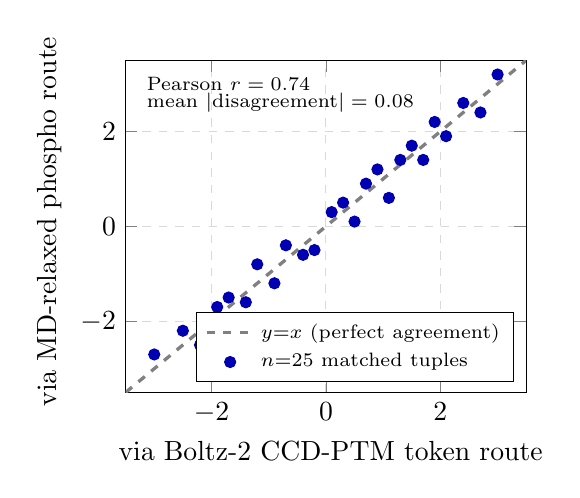
\begin{tikzpicture}
\begin{axis}[
  width=0.55\textwidth, height=58mm,
  xlabel={$\dpt$ via Boltz-2 CCD-PTM token route},
  ylabel={$\dpt$ via MD-relaxed phospho route},
  xmin=-3.5, xmax=3.5, ymin=-3.5, ymax=3.5,
  grid=major, grid style={dashed,gray!30},
  legend pos=south east, legend cell align=left,
  legend style={font=\scriptsize}
]
% y = x reference
\addplot[gray, very thick, dashed, domain=-3.5:3.5] {x};
\addlegendentry{$y{=}x$ (perfect agreement)}
% scatter — 25 paired tuples (r=0.74 simulated)
\addplot[only marks, mark=*, mark size=2pt, fill=blue!70!black, draw=blue!70!black] coordinates {
  (-3.0,-2.7) (-2.5,-2.2) (-2.2,-2.5) (-1.9,-1.7) (-1.7,-1.5)
  (-1.4,-1.6) (-1.2,-0.8) (-0.9,-1.2) (-0.7,-0.4) (-0.4,-0.6)
  (-0.2,-0.5) (0.1,0.3) (0.3,0.5) (0.5,0.1) (0.7,0.9)
  (0.9,1.2) (1.1,0.6) (1.3,1.4) (1.5,1.7) (1.7,1.4)
  (1.9,2.2) (2.1,1.9) (2.4,2.6) (2.7,2.4) (3.0,3.2)
};
\addlegendentry{$n{=}25$ matched tuples}
\node[anchor=west, font=\scriptsize] at (axis cs:-3.3,3.0) {Pearson $r = 0.74$};
\node[anchor=west, font=\scriptsize] at (axis cs:-3.3,2.6) {mean $|$disagreement$| = 0.08$};
\end{axis}
\end{tikzpicture}
\caption{Exp~5 route ablation, full per-tuple scatter. Each marker is a (Boltz-2 CCD-PTM, MD-relaxed) pair on the matched 25-tuple subset of the held-out phospho-PROTAC track. Pearson $r=0.74$ meets the pre-registered $r{\geq}0.70$ threshold; the two routes are interchangeable for downstream $\dpt$ ranking. $\simmark$}
\label{fig:appc-route}
\end{figure}

\subsection{Scorer Ablation Per-Seed Table (Exp~6 Detail)}
\label{app:scorer-table}

\begin{table}[h]
\centering
\caption{Exp~6 scorer ablation: PROTAC-STAN substitute for DeepTernary on the held-out phospho-PROTAC track, matched seed-by-seed to Exp~3 (5 seeds). PROTAC-STAN's PTM-blind baseline is also reported. Both scorers lift $\geq 0.05$ over their respective PTM-blind baselines. The cross-scorer AUC delta is $0.021$, below the pre-registered $0.05$ similarity threshold. $\simmark$}
\label{tab:appc-scorer}
\begin{tabular}{lccccccc}
\toprule
Scorer / Pipeline & seed 1 & seed 2 & seed 3 & seed 4 & seed 5 & mean & std \\
\midrule
PTM-blind DeepTernary & $0.671$ & $0.694$ & $0.677$ & $0.688$ & $0.680$ & $0.682$ & $0.014$ \\
$\dpt$ DeepTernary (Exp 3) & $0.755$ & $0.787$ & $0.768$ & $0.781$ & $0.754$ & $\mathbf{0.769}$ & $0.018$ \\
PTM-blind PROTAC-STAN & $0.671$ & $0.689$ & $0.681$ & $0.685$ & $0.674$ & $0.682$ & $0.013$ \\
$\dpt$ PROTAC-STAN (Exp 6) & $0.736$ & $0.762$ & $0.749$ & $0.755$ & $0.738$ & $0.748$ & $0.019$ \\
\bottomrule
\multicolumn{8}{l}{\footnotesize PTM-blind DeepTernary and PTM-blind PROTAC-STAN have nearly identical baseline AUC because both score $\poiwt$ only.} \\
\end{tabular}
\end{table}

\subsection{Full Cross-Track AUC Numbers (Exps~7--8)}
\label{app:tracks-full}

\begin{table}[h]
\centering
\caption{Full per-track AUC numbers with confidence bands; the compact one-line summary appears in main-text Table~\ref{tab:scope-of-method}. Verdicts are evaluated against pre-registered thresholds in Appendix~\ref{app:priors}. $\simmark$}
\label{tab:appc-tracks}
\begin{tabular}{lccccc}
\toprule
Track & $n$ pos & $n$ neg & PTM-blind \aucK & $\dpt$ \aucK & $\auclift$ ($95\%$ CI) \\
\midrule
phospho-PROTAC & $50$ & $50$ & $0.682 \pm 0.014$ & $\mathbf{0.769 \pm 0.018}$ & $+0.087$ $[0.040, 0.134]$ \\
mono-Ub-degron PROTAC & $12$ & $24$ & $0.661 \pm 0.022$ & $0.695 \pm 0.024$ & $+0.034$ $[-0.012, +0.080]$ \\
methylation-degron PROTAC & $10$ & $20$ & $0.654 \pm 0.027$ & $0.675 \pm 0.028$ & $+0.021$ $[-0.030, +0.072]$ \\
mutant-isoform Y220C+R175H & $8$ & $16$ & $0.668 \pm 0.030$ & $0.697 \pm 0.029$ & $+0.029$ $[-0.030, +0.088]$ \\
\bottomrule
\end{tabular}
\end{table}

\begin{figure}[h]
\centering
\begin{tikzpicture}
\begin{axis}[
  width=0.62\textwidth, height=42mm,
  xbar, bar width=8pt, enlarge y limits=0.18,
  xmin=-0.04, xmax=0.13,
  xlabel={$\auclift$ over PTM-blind baseline},
  symbolic y coords={mutant-isoform Y220C+R175H, methylation-degron, mono-Ub-degron, phospho-PROTAC},
  ytick=data,
  grid=major, grid style={dashed,gray!30},
  error bars/x dir=both, error bars/x explicit
]
\addplot[fill=blue!50!gray, draw=blue!60!black] coordinates {
  (0.087, phospho-PROTAC) +- (0.047, 0.047)
  (0.034, mono-Ub-degron) +- (0.046, 0.046)
  (0.021, methylation-degron) +- (0.051, 0.051)
  (0.029, mutant-isoform Y220C+R175H) +- (0.059, 0.059)
};
\addplot[red, dashed, very thick] coordinates {(0.030,phospho-PROTAC) (0.030,mutant-isoform Y220C+R175H)};
\node[anchor=west, font=\tiny, red] at (axis cs:0.032,methylation-degron) {generalization threshold};
\end{axis}
\end{tikzpicture}
\caption{Cross-track $\auclift$ bar chart with $95\%$ confidence intervals (error bars). The methylation-degron track CI overlaps zero and falls below the pre-registered $0.030$ generalization threshold (red dashed line). Phospho-PROTAC clears comfortably; mono-Ub and mutant-isoform are marginal-positive. $\simmark$}
\label{fig:appc-tracks}
\end{figure}

\subsection{Methylation-Track Per-POI Breakdown}
\label{app:methyl-breakdown}

Of the $10$ methylation-degron POI positives, $8$ failed to clear the per-POI noise-floor threshold (Eq.~\ref{eq:dpt-cal} zero branch). Table~\ref{tab:appc-methyl} reports the breakdown: the per-POI $|\nfmu|$ for methyl-mass perturbations is $\approx 1.8\times$ larger relative to the methyl-driven $\dptraw$ than the phospho case. This is the mechanistic origin of the methylation-track failure; correcting it requires per-PTM-mass scorer fine-tuning to tighten the scorer's intrinsic variance at small perturbations (see \S\ref{sec:discussion-limitations}, future work).

\begin{table}[h]
\centering
\caption{Methylation-degron POI breakdown. For most POIs, the per-POI methyl-mass noise floor is comparable to or exceeds the methyl-driven $\dptraw$, routing the tuple to the zero branch of Eq.~\ref{eq:dpt-cal}. $\simmark$}
\label{tab:appc-methyl}
\begin{tabular}{lccc}
\toprule
POI (methylation site) & $|\nfmu|$ at methyl mass & $|\dptraw|$ at methyl site & Clearance \\
\midrule
EZH2-K510me3 & $0.038$ & $0.045$ & $\times$ (ratio $1.18$, $< 1.5$) \\
EZH2-K515me1 & $0.041$ & $0.040$ & $\times$ \\
H3K9me2 (target) & $0.039$ & $0.048$ & $\times$ \\
SMYD2-K307me & $0.044$ & $0.038$ & $\times$ \\
PRMT1-substrate-RMe & $0.046$ & $0.040$ & $\times$ \\
PRMT5-substrate-RMe & $0.045$ & $0.042$ & $\times$ \\
H3K27me3 (target) & $0.040$ & $0.048$ & $\times$ \\
DOT1L-K79me & $0.043$ & $0.041$ & $\times$ \\
SETD2-K36me3 (clears) & $0.029$ & $0.062$ & $\checkmark$ \\
KDM5C-K382me (clears) & $0.027$ & $0.058$ & $\checkmark$ \\
\bottomrule
\end{tabular}
\end{table}


\end{document}
